
ElecSIM has been designed for ease of use to enable non-experts to rapidly test policies and observe the outcomes of various scenarios such as demand growth. The user is able to input exogenous variables such as fuel costs, carbon taxes, number and type of power plants, power plant costs and electricity demand. This allows for the initialisation of different countries and scenarios to be tested.


\subsection{Overview}

\begin{figure}[b]
	\centering
	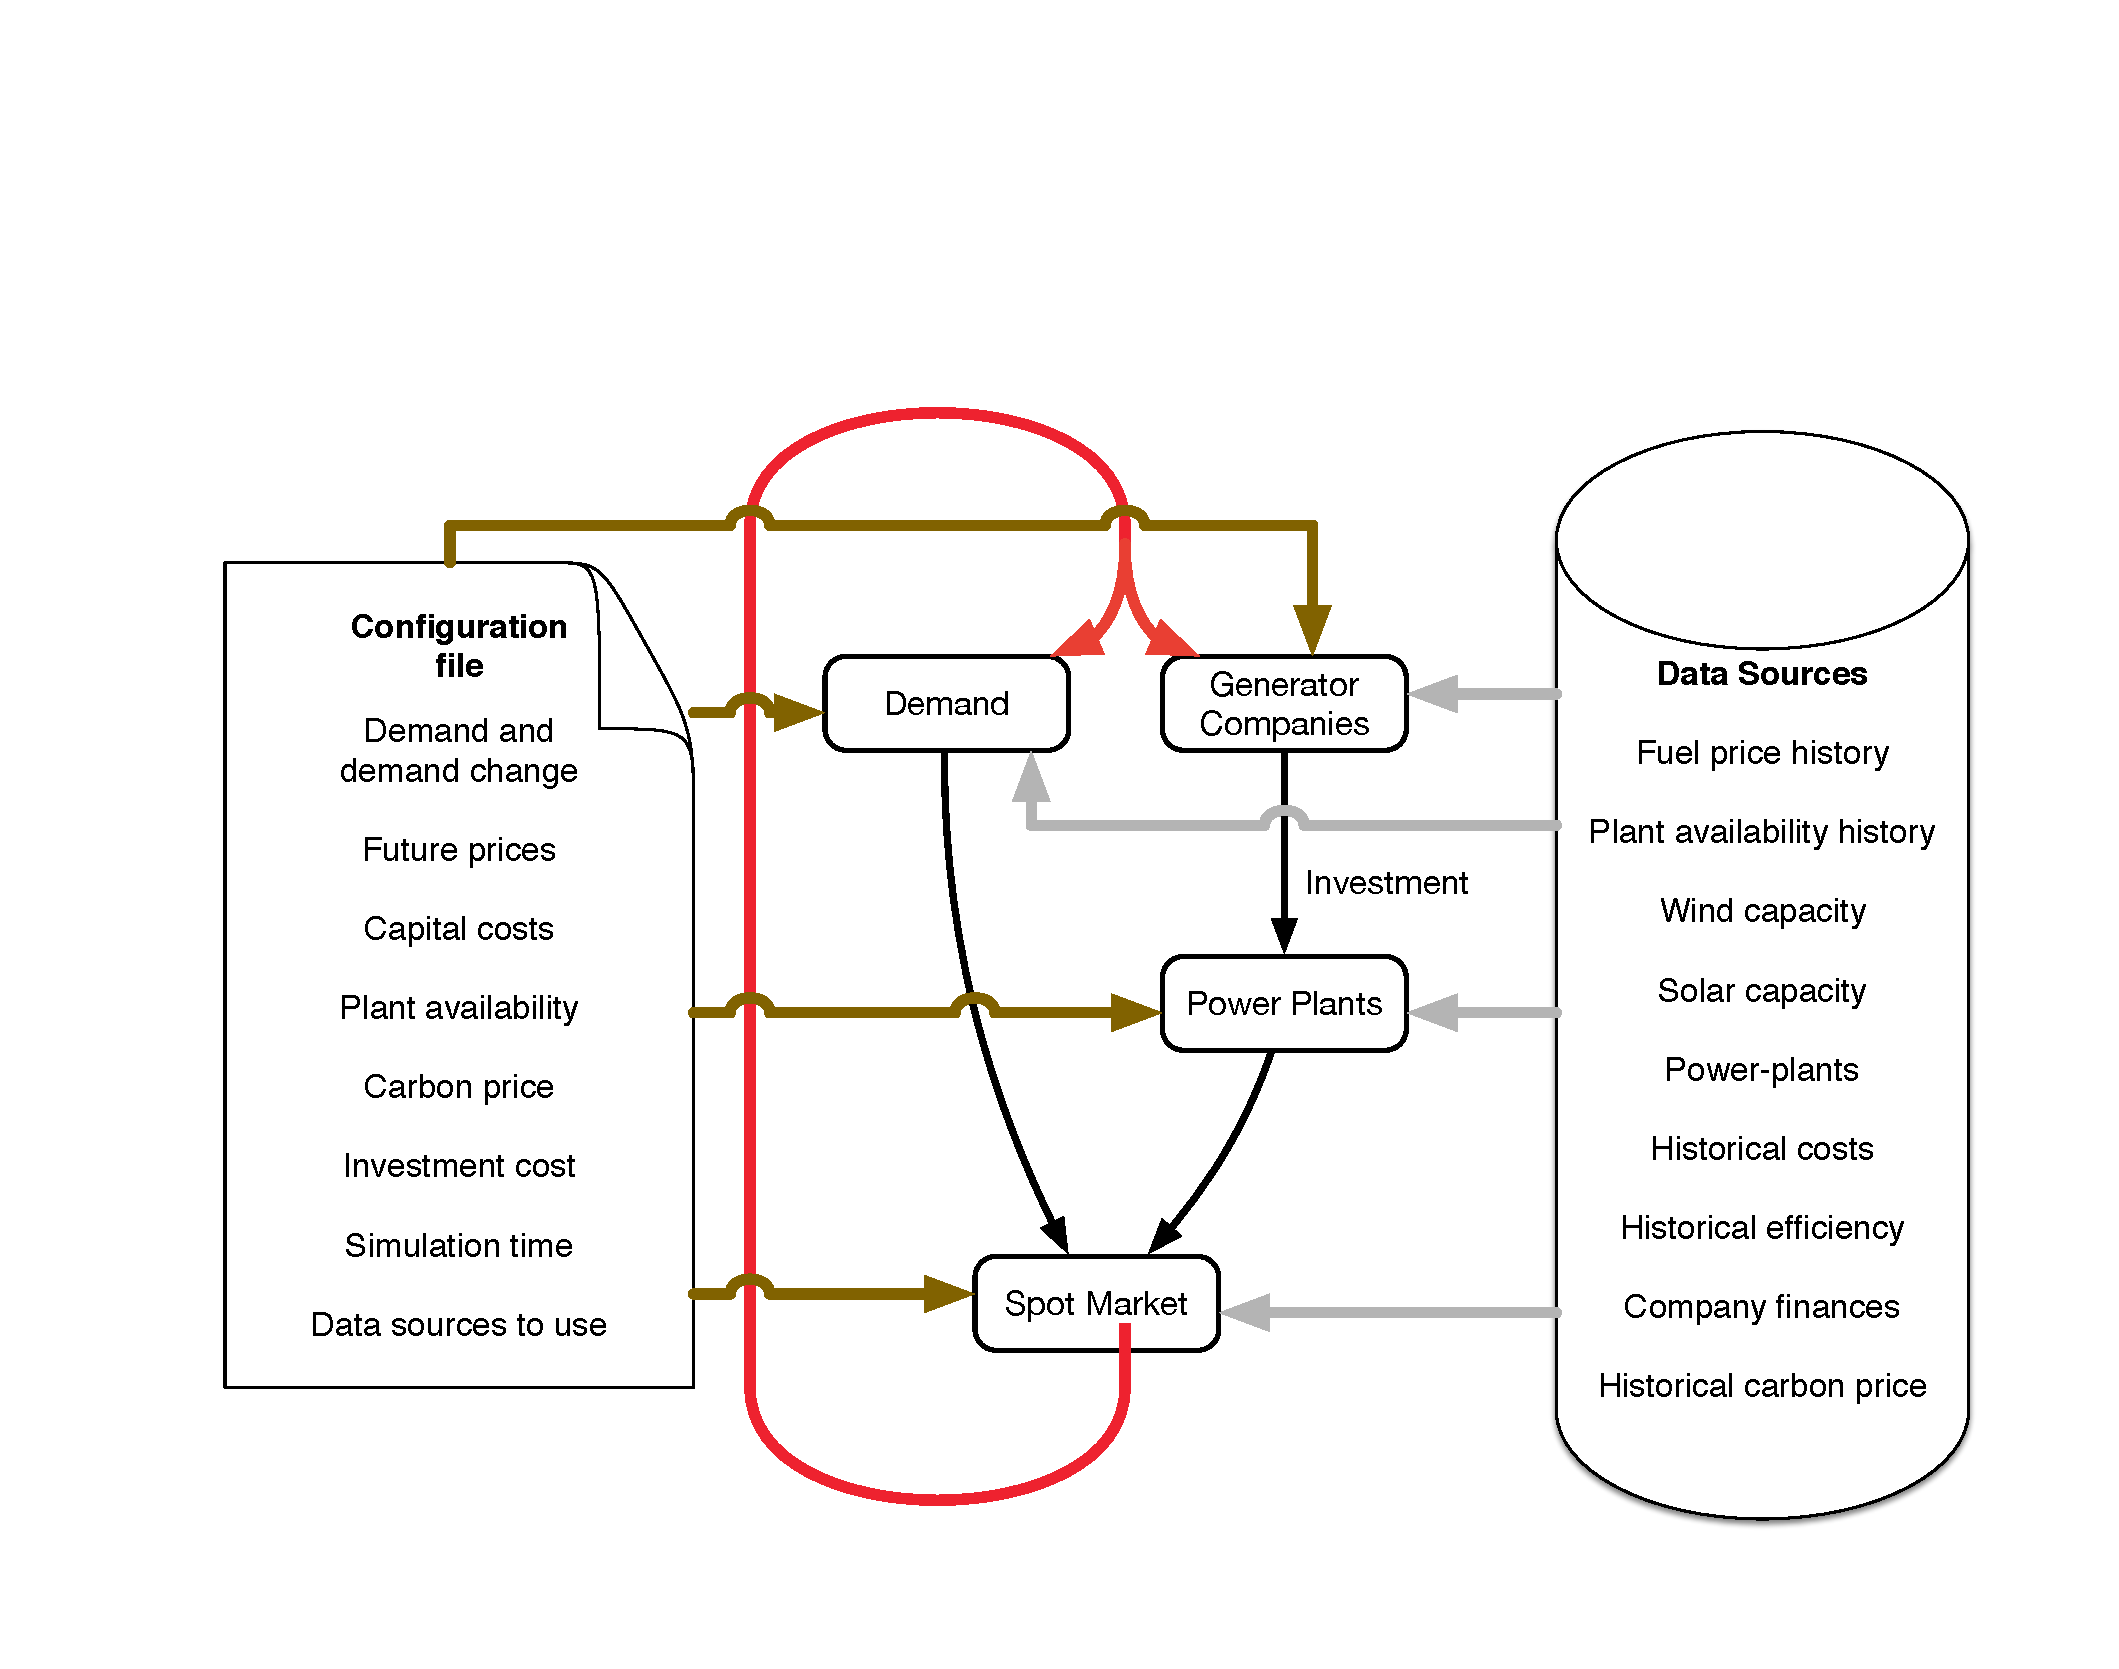
\includegraphics[width=0.97\linewidth]{figures/System_overview}
	\caption{High level system overview demonstrating fundamental parts of ElecSIM.}
	\label{fig:systemoverview}
\end{figure}




ElecSIM is made up of five fundamental parts: the agents, which are split up into demand and generation companies (GenCos); power plants, which are owned by the GenCos; a Power Exchange, which controls a spot market to match GenCo owned power plants with electricity demand; the world in which these agents and market exist; and the data for parametrisation.

A schematic of ElecSIM is displayed in Figure \ref{fig:systemoverview} which displays these four fundamental sections and demonstrates how they interact. The main components are discussed below:

\subsubsection{Data parametrisation} To parametrise the world ElecSIM contains a configuration file and a collection of data sources. These data sources contain information such as historical fuel prices, historical plant availability, wind and solar capacity, power plant costs, historical costs, historical efficiency, company finances and historical carbon price. This is data that does not change from scenario to scenario, however can vary between countries.

The configuration file allows for rapid changes to test different hypothesis and scenarios, and points to previously mentioned data sources. The configuration file enables the changing of demand growth and shape,  future fuel and carbon prices, capital costs, plant availability, investment costs and simulation time. These data is used to calibrate the world.

\subsubsection{Demand Agent}
The demand agent is a simplified representation of aggregated demand in a particular country. The demand is represented as a load duration curve. An example load duration curve for a year is demonstrated in Figure \ref{fig:loaddurationcurve}. A load duration curve is an arrangement of all load levels in descending order of magnitude, where the lowest segment demand demonstrates baseload (ie. 100\% of time), and the highest segment represents peak demand. Each year, the demand agent multiplies the percentage of change in demand with each segment of the load duration curve. Therefore, whilst total demand changes between years, the ratio between each segment of the load duration curve is assumed not to change.

\begin{figure}
	\centering
	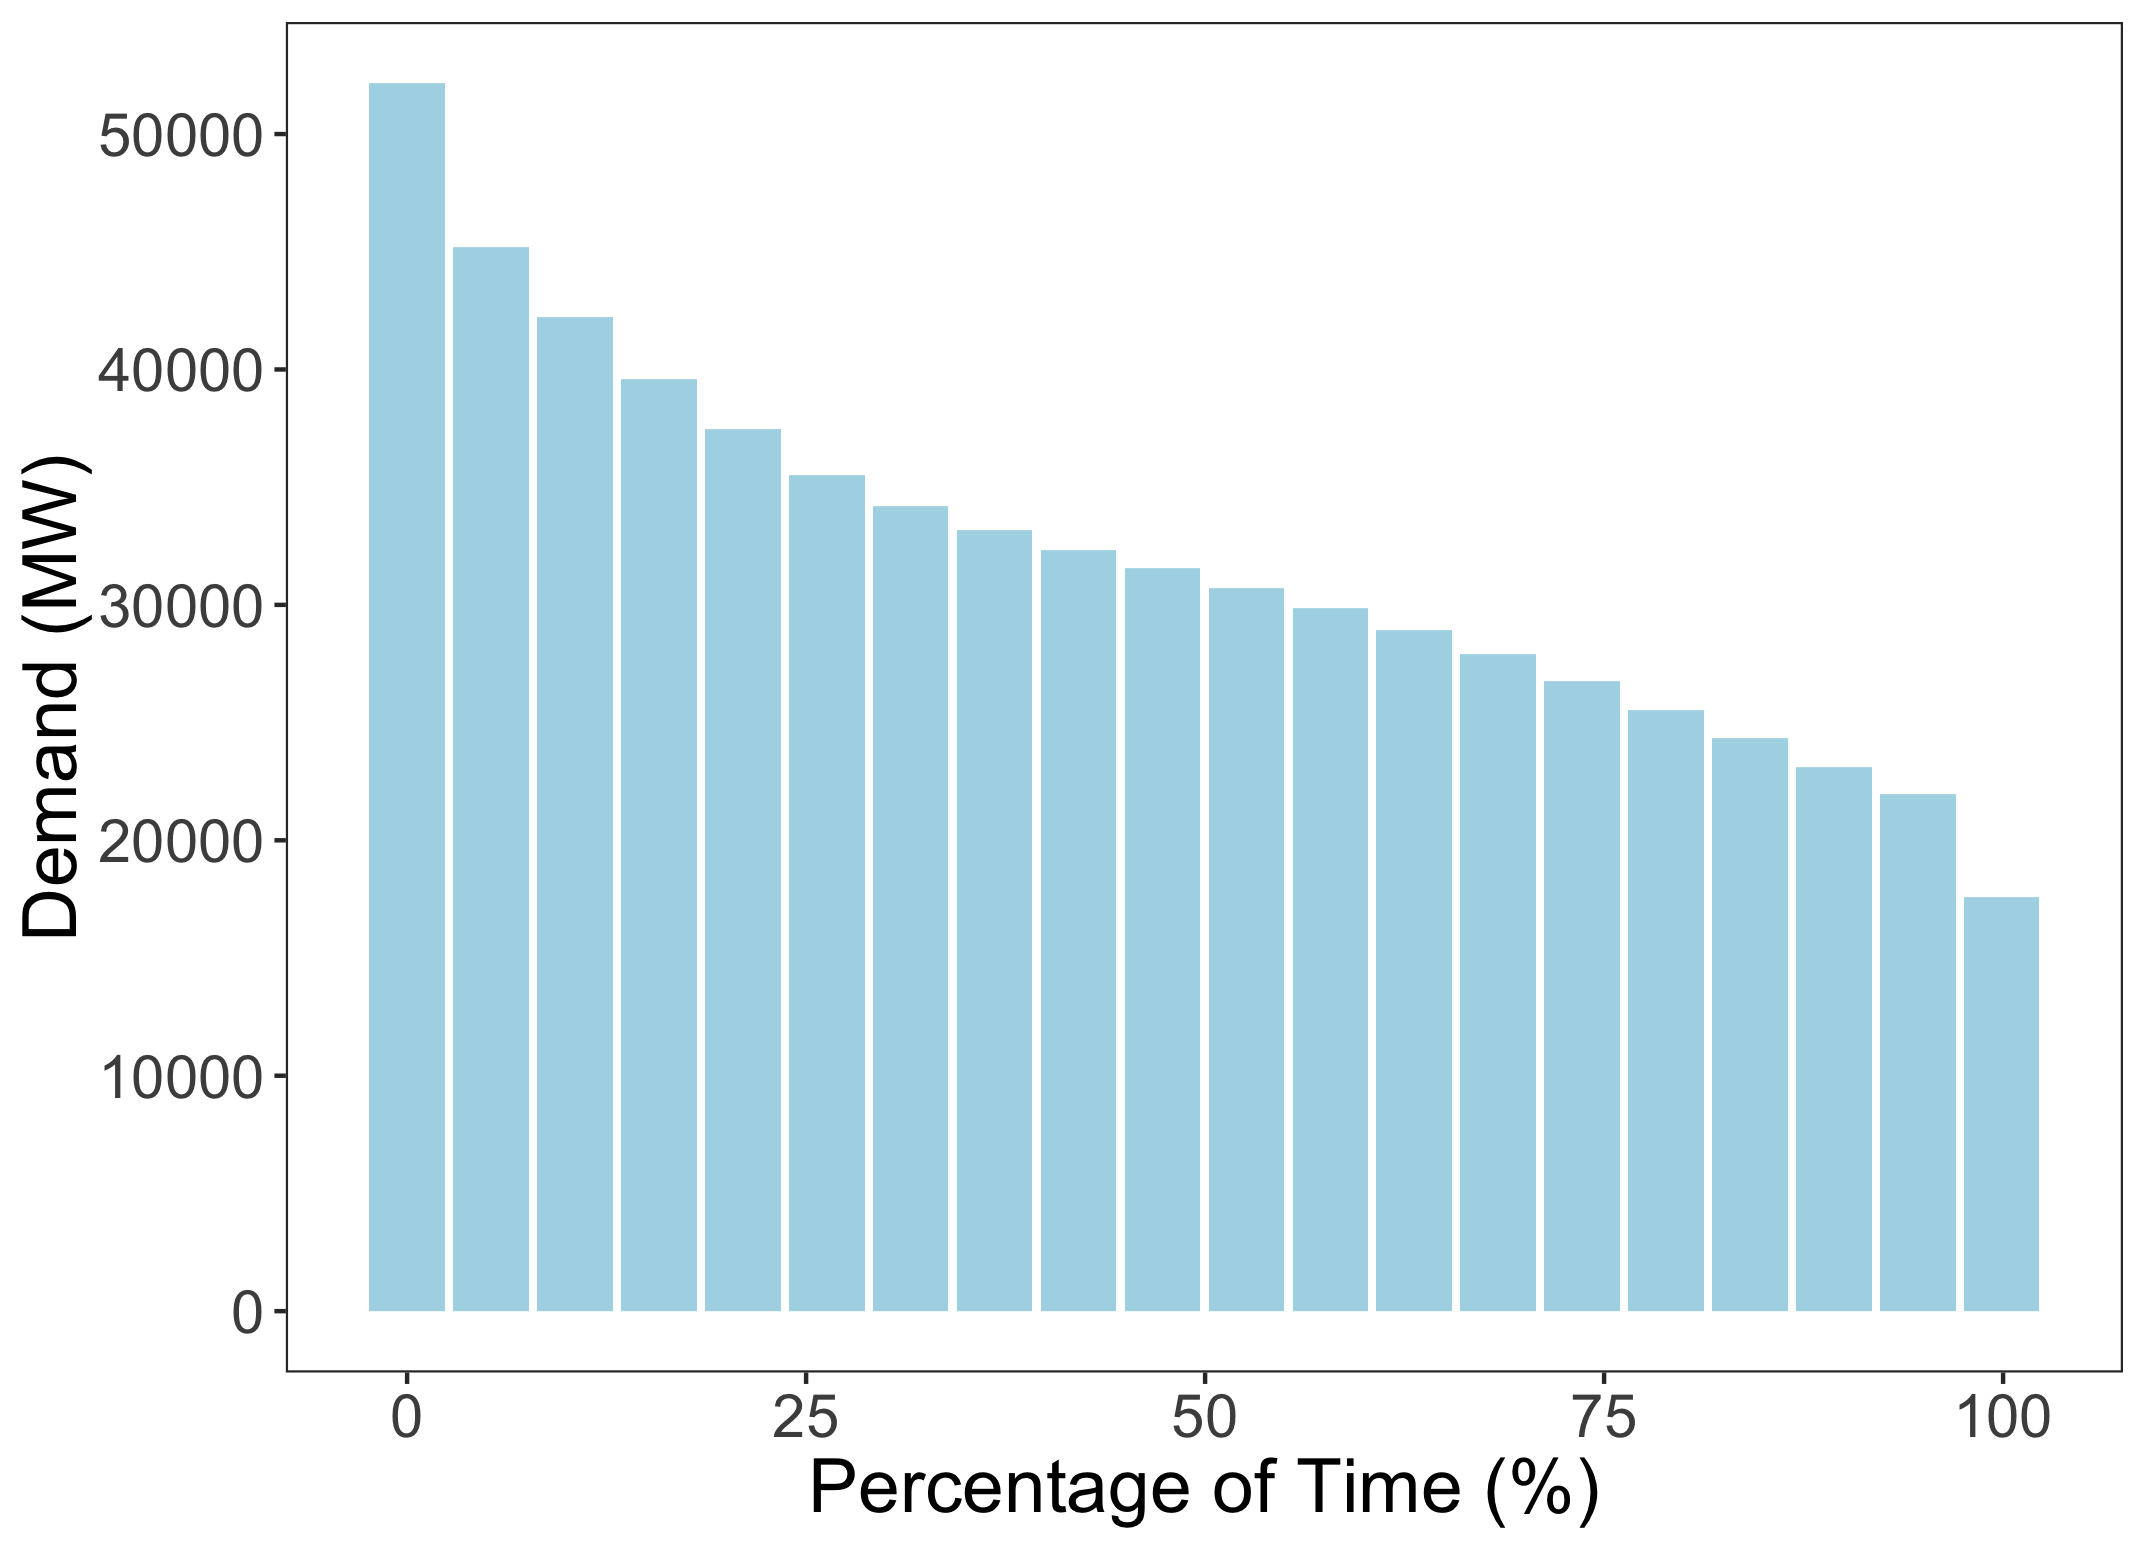
\includegraphics[width=0.95\linewidth]{figures/load_duration_curve}
	\caption{Example load duration curve in a single year.}
	\label{fig:loaddurationcurve}
\end{figure}

As per Chappin \textit{et al.} \cite{Chappin2017}, we modelled the load duration curve of the electricity demand for one year with twenty segments. Twenty segments enabled us to capture the varying demand of electricity throughout the year to a high enough degree of accuracy, whilst also reducing computational complexity. 


\subsubsection{Generation Company Agents} The GenCos have two main functions. Investing in power plants and making bids to sell their electricity each year for every one of their power plants. We will first focus on the buying and selling of electricity using a Power Exchange, and then cover the investment algorithm used by GenCos.

\subsubsection{Electricity Market} \label{sssec:electricity_market} A simulated electricity market is run every year, where electricity is bought and sold on an electricity spot market. Figure \ref{fig:powermarket} displays the market process for each segment of demand. Power plants bid the short run marginal cost (SRMC) of each power plant. SRMC is the price that it costs a generator to sell a unit of electrical power (1MWh) excluding fixed and capital costs. 

The power exchange sorts bids in order of price, as is shown in Figure \ref{fig:powermarket}, and accepts the lowest bids until supply meets demand. Once supply meets demand, the spot price or system marginal price (SMP) is paid to all generators regardless of their initial bid. It is for this reason that generators are motivated to bid their SRMC, to ensure that their generator is being utilised, and reducing the risk of over bidding and not being selected.

Higher segments of demand command higher prices, due to more expensive generators being selected to meet demand. This leads to a price duration curve.
 

\begin{figure}
	\centering
	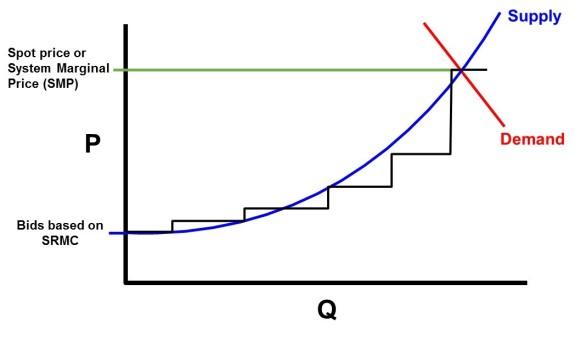
\includegraphics[width=1\linewidth]{figures/power_market}
	\caption{Power exchange clearing \cite{nuclear_economics_consulting_group_2019}.}
	\label{fig:powermarket}
\end{figure}

\subsubsection{Investment}

Investment in power plants is made based upon a net present value (NPV) calculation. NPV is a summation of the present value of a series of present and future cash flow. NPV provides a method for evaluating and comparing investments with cash flows spread over many years, making it suited to evaluating power plants which have a long lifetime. A positive NPV means that the projected investment exceeds the anticipated costs, and is therefore profitable. NPV is based upon the fact that current cash flow is worth more than future cash flow. This is due to the fact that money today can be invested and have a rate of return. This means that, for example \$50,000 today is worth more than \$50,000 in 10 years time. The value in which future cash flow is worth less than present cash flow is discounted by the discount rate.

Equation \ref{eq:npv_eq} is the calculation of NPV. Where $t$ is the year of the cash flow, $i$ is the discount rate, $N$ is total number of periods, or lifetime of power plant, and $R_t$ is the net cash flow (cash inflow minus cash outflow) at time $t$.

\begin{equation} \label{eq:npv_eq}
NPV(i, N) = \sum_{t=0}^{N}\frac{R_t}{(1+t)^t}
\end{equation}

A discount rate set by a firm's weighted average cost of capital (WACC) is often used \cite{KincheloeStephenC1990TWAC}. WACC is the rate that a company is expected to pay on average for its stock and debt. Therefore, if the income is higher than the WACC then the NPV is positive, and becomes a worthwhile investment. However, it is often believed that a higher rate than the WACC should be selected to adjust for differing risk profiles, opportunity cost and rate of return desired.

Data is available for average WACC for power plants, and can be set in the configuration file. However, to account for differing risk profiles, opportunity costs, rate of return desired and a WACC based on companies' relative credit risk, we have sampled differences in discount rates from the mean WACC with a Gaussian distribution with a standard deviation of $\pm3\%$. This was chosen to give sufficient variance between GenCos whilst remaining close to the mean set by the user.

To calculate the expected return per year of a power plant, an understanding of future market conditions is required. Future market conditions are dependent on demand and costs that would be incurred by the GenCo based upon each prospective investment. We simplify this calculation by forecasting $N$ years into the future, which can be selected by the user. We assume that this year is representative of each year of a power plant's lifetime.

As in the real world, GenCos have imperfect information, and therefore must forecast expected demand, fuel prices, carbon price and electricity sale price. This achieved by fitting functions to historical data. Each GenCo is different in that they will use differing historical time periods of data to forecast in the future. The distribution of this is configurable in the configuration file, referred to in Figure \ref{fig:systemoverview}.

Fuel price and carbon price are forecast using a linear regression. Demand, however, is first forecast using an exponential function, to take into account compounded growth. If a reasonable fit for historical demand data can not be found with optimisation, linear regression is used.

This forecast data is then used to simulate a market $N$ years into the future using the same electricity market algorithm that is detailed in Section \ref{sssec:electricity_market}. We simulate a market based on the expected bids -- based on SRMC -- that every operating power plant will make. This includes the removal of plants that will be past their operating period, and the introduction of plants that are in construction or pre-development stages. 

However, there may be scenarios where demand is forecast to grow significantly, and limited investments have, at this point, been made to meet demand at $N$ years into the future. The expected price, would therefore be calculated to be that of lost load. Where lost load is defined as the price customers would be willing to pay to avoid disruption in their electricity supply, and is typically much higher than average prices. To avoid GenCos from predicting that large profits will be made, and under the assumption that further power plant investments will be made by other GenCos in the future, the lost load price is replaced with a predicted electricity price using a linear regression based on prices at lower points of the demand curve. If zero segments of demand are met (ie. total supply of generators is smaller than baseload), then the lost load price is used to encourage significant investment. If only a single segment of demand is met then the price of this demand segment is chosen. The lost load price can be configured in the configuration file.

Once expected fuel prices, carbon price, discount rate, and expected sale price of electricity are all forecast, the NPV can be calculated. GenCos must typically provide a certain percentage of upfront capital, with the rest coming from investors in the form of stock and shares or debt (WACC). The percentage of upfront capital, or down payment, is set at $25\%$, but can be customised by the user in the configuration file. The GenCos then invest in the power plant with the highest NPV that they can afford, and this is repeated until they can no longer afford any more plants. We make this assumption as the NPV calculation provides information based upon risk profile and required rate of return.

\subsection{Power Plant Parameters}\label{ssssec:powerplantparameters}



The estimation of power plant parameters is critical to electricity market models. Costs form an important element of markets and investment, and publicly available data for power plant costs for individual countries can be scarce. Thus, extrapolation and interpolation is required to estimate costs for power plants of differing sizes, types and years of construction.

We enable users to initialise costs relevant to their particular country. They can provide highly detailed cost parameters, with the parameters shown in Table \ref{table:parameter_notation}, or an average cost per MWh produced over the lifetime of a plant, also known as levelised cost of electricity (LCOE).

The parameters in Table \ref{table:parameter_notation} are detailed here: Efficiency ($\eta$) is defined as the percentage of energy from fuel that is converted into electrical energy. Operating period ($OP$) is the total period in which a power plant is in operation. Pre-development period ($P_D$) and pre-development costs ($P_C$) include the time and costs for pre-licensing, technical and design, as well as costs incurred due to regulatory, licensing and public enquiry. The construction period ($C_D$) and construction costs ($C_C$) are incurred during the development of the plant, excluding network connections. The infrastructure costs ($I_C$) are the costs incurred by the developer in connecting the plant to the electricity or gas grid. Fixed operation \& maintenance costs ($F_C$) are costs incurred in operating the plant that do not vary based on plant output. Variable operation \& maintenance ($V_C$) costs are costs incurred in operating the plant that do depend on generator output \cite{Ltd2016}.



\begin{table}[h]
	\centering
	\csvautobooktabular{tables/notation_formated.csv}
	\caption{Parameter notation. (Whilst the unit of currency displayed is \textsterling, this can easily be changed to suit specific needs eg. \$, \texteuro)}
	\label{table:parameter_notation}
\end{table}
\addtolength{\textfloatsep}{-0.2in}

Precise data is often available only for specific sized plants. Estimating the individual costs of power plants between two known capacities is achieved through linear interpolation of each parameter. When the plant to be estimated falls outside of the range of known data points, the closest data point is used. For example, the parameters of a $1,500$MW combined cycle gas plant (CCGT) are estimated to be the same as a $1,200$MW CCGT plant if the $1,200$MW plant was the largest available data point. 

If specific parameters are not known (those referred to in Table \ref{table:parameter_notation}), then the LCOE can be used for parameter estimation, provided that these parameters are available for a single instance of each type of power plant. This is achieved through linear optimisation, with constraints available for each of the parameters. These constraints can be set by the user, enabling, for example, varying operation and maintenance costs per country as a fraction of the levelised cost of electricity.


In addition to cost parameters, the availability and capacity factors are required to fully parametrise power plants. Availability is the percentage of time that a power plant could possibly produce electricity over a given time period. Availability can be reduced by forced and planned outages. Historical data is also required, due to the fact that older plants have lower availability factors than newer plants.

Capacity factor is the actual electrical energy produced over a given time period divided by the maximum possible electrical energy it could have produced. In contrast to availability, capacity factor can be impacted by regulatory constraints, market forces and resource availability. For solar and wind, capacity factors can change significantly with time. Higher capacity factors are common for solar installations in the summer, and lower in winter for example \cite{Stoft2002}. 

To model the intermittency of wind and solar power we allow them to contribute only a certain percentage of their total capacity (nameplate capacity) for each load segment. This percentage is based upon empirical wind and solar capacity factors, relating demand to average capacity. This is due to the fact that there is a correlation between demand and wind speed, as well as with solar irradiance. The requirement of storage to provide constant electricity from intermittent resources is an important issue. However, due to the fact that ElecSIM takes yearly time steps, we are unable to model short term variability in electricity demand. We also, do not model long-term storage due to its currently limited ability. 

When initialised, the variable operation and maintenance costs are selected from a uniform distribution, with the ability for the user to set maximum percentage increase or decrease. A uniform distribution was chosen to capture the large deviations that can occur in variation of variable operation and maintenance, especially over a long time period. By doing this, the variance in costs between individual power plants for processes such as preventative and corrective maintenance, labour costs and skill, health and safety and chance are different per plant instant.  

Whilst fuel price is controlled by the user, there is inherent volatility in fuel price within a single year. To take into account this variability, an ARIMA model was fit to historical gas and coal price data. The standard deviation of the residuals was used to model the deviation of fuel price that a generation company will buy fuel at in a given year. This takes into account differences in hedging strategies and the process of luck between competing generation companies.

With historical power plants which have been refurbished, we sample their initialisation randomly between 15 years prior to initialisation year and the initialisation year. This is done because there is rarely a comprehensive data set on when plants are refurbished. 15 years was chosen due to the fact that plants often have an operating period of 25 years, and therefore 15 years allowed for sufficient variance in results, whilst keeping plants in operation.

\subsubsection{ElecSIM World}

Figure \ref{fig:lowlevelsystem} demonstrates the world and how it co-ordinates data and processes. It contains information on every single GenCo, Power Exchange, and runs processes. The world also contains information on the year number and collects simulation data.

The world brings together power plant data on one side, and demand data on the other. The investment decisions are based upon future demand and power plant costs. The merit order bids are based upon the investment decisions made and power plant costs.

Exogenous variables include fuel and \ce{CO2} prices as well as demand growth. Once the data is initialised, the world calls on the Power Exchange to operate the yearly electricity spot market.

%The world contains the functionality to dismantle old plants once they have reached the end of their lifetime. Power plants are taken out of service if they have not sold any electricity in the past 7 years, which is configurable in the configuration file. We decided upon this due to the fact that power generators have high, sunk capital costs, which often have high demolition costs. We assume, therefore, that generator companies are willing to wait circa $\frac{1}{4}$ of their lives to see if a pay-out occurs due to the breakdown of competing power plants, increasing demand, or governmental support in the form of a carbon tax increase or reduction.

The world also settles the accounts of the GenCos, by paying bids, and removing operating and capital costs as well as loan and dividend payments.

\begin{figure*}
	\centering
	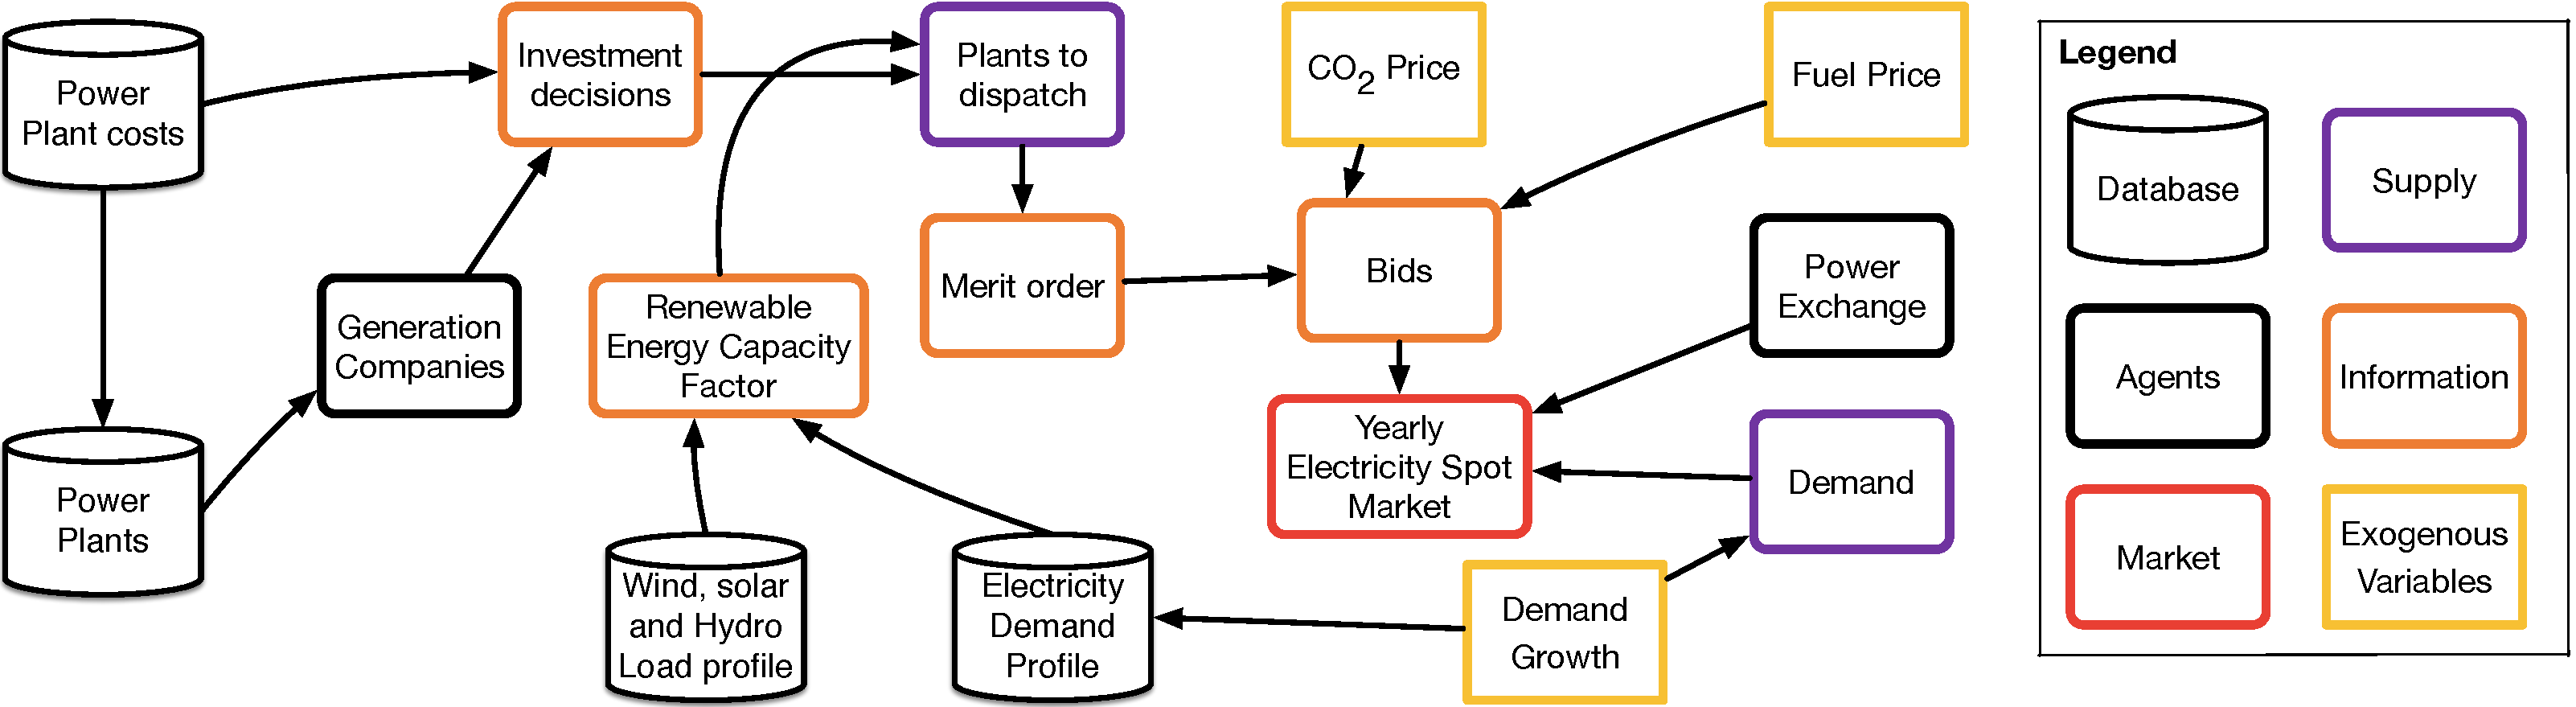
\includegraphics[width=0.97\linewidth]{figures/low_level_system}
	\caption{ElecSIM simulation overview}
	\label{fig:lowlevelsystem}
\end{figure*}


%GenCos  invest in power plants based on the highest positive net present value (NPV). Bids are made for each power plant based on the power plants short run marginal cost. A Power Exchange operator matches these bids with demand in merit order. 



%\begin{figure}[h]
%	\begin{center}
%		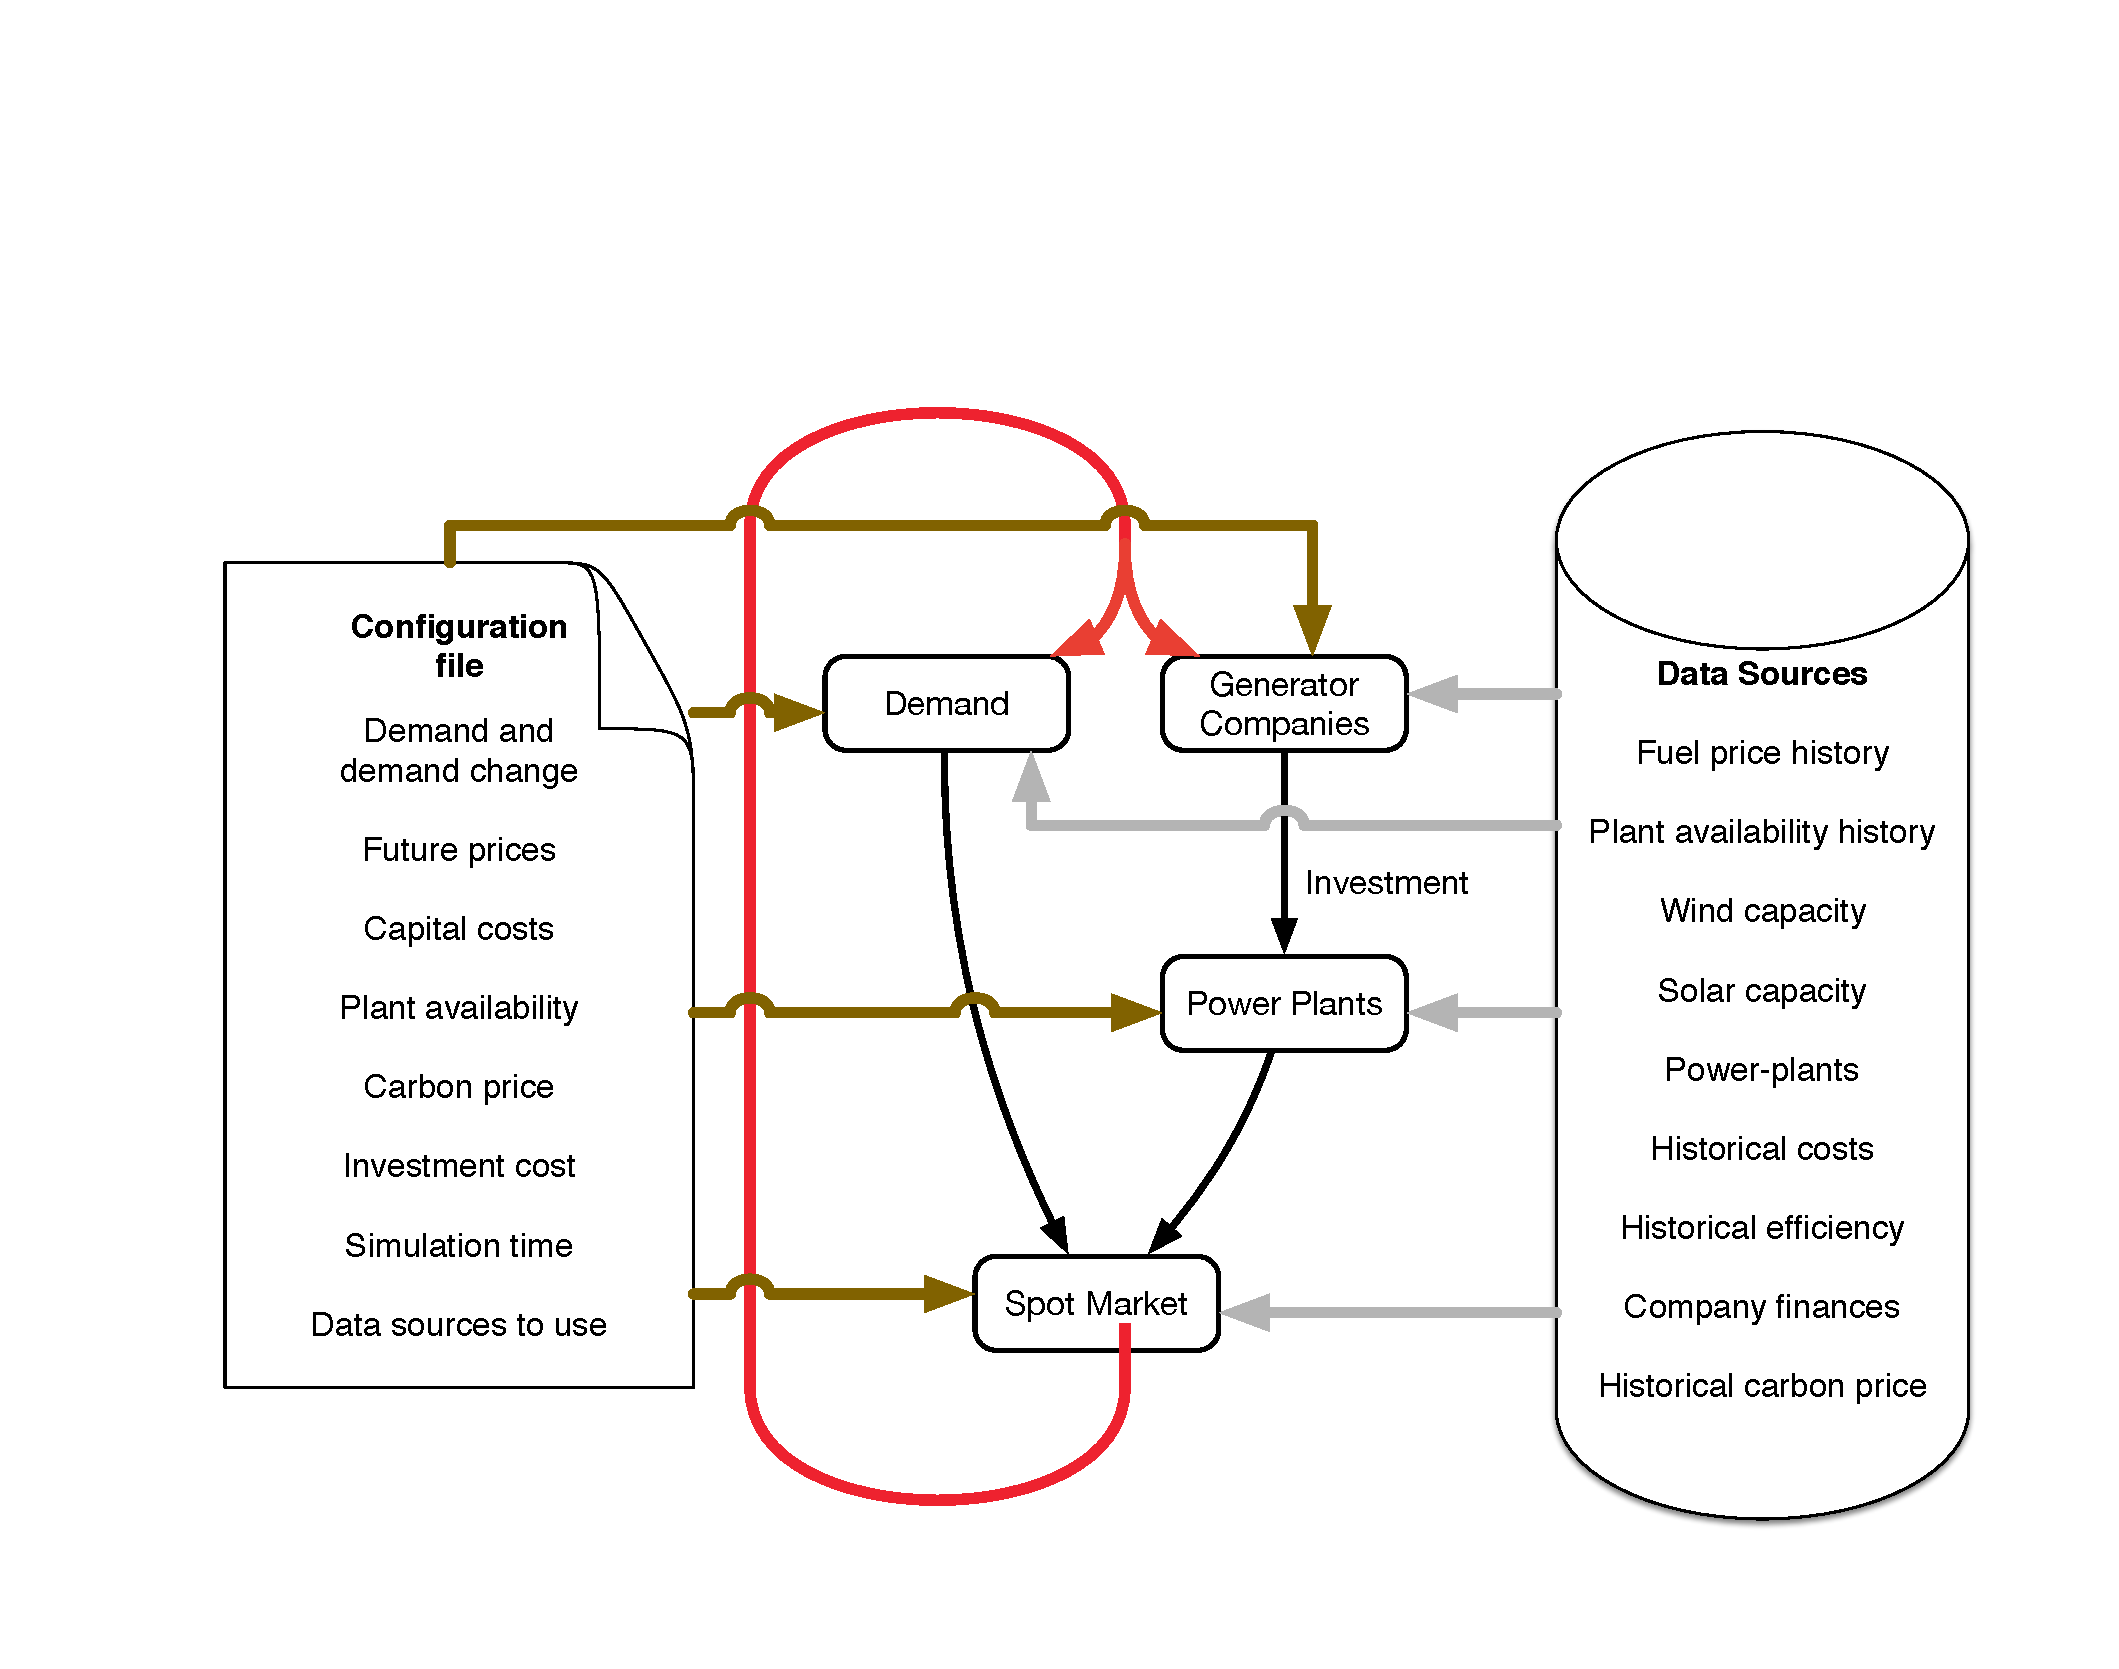
\includegraphics[width=0.5\textwidth]{figures/System_overview.pdf}
%		\caption{ElecSIM simulation overview.}
%		\label{fig:system_overview}
%	\end{center}
%\end{figure}




\subsection{UK Case Study}

Here we study a realisation of ElecSIM, which we calibrated to the United Kingdom.

\subsubsection{Exogenous Inputs}

To model variance in gas and coal prices we used data from \cite{coalprices,gasprices}. Calibration of the load duration curve was taken from \cite{gbnationalgridstatus_2019}.

Historical EU ETS carbon price was taken from \cite{jones_moore_macdonald_macdonald_buckley_macdonald_2019}. The EU ETS is the EU emissions trading scheme, which limits total carbon emissions within the EU area.

\subsubsection{Power Plant Parameters}

ElecSIM's power generation costs are initialised using the UK government Department for Business, Energy and Industrial Strategy (BEIS) power plant generation report \cite{Department2016}. This contains information on power plants found in Table \ref{table:parameter_notation}.

For historical power plants, we used historical costs of Levelised Cost of Energy (LCOE) \cite{Dale2013}, from the International Energy Agency and International Renewable Energy Agency energy cost reports, localised to the UK \cite{IEA2015,IRENA2018}. In this realisation, each parameter was scaled linearly going from the modern LCOE calculated from the BEIS report, to attain the relevant historical LCOE. Historical plant efficiency was taken into account for gas and coal power plants using data from the USA \cite{EIA2013}.

Outages are modelled by using availability data of gas, coal, photovoltaic, offshore and onshore power generators \cite{Ltd2016, Hunt2015, carroll-j}. Historical availabilities are modelled for older gas, coal and hydro power plants \cite{AlbertaSystemElectricOperator2016}.

Capacity factors were taken as an average of the UK for solar and wind \cite{Pfenninger2016, Staffell2016}.






\subsubsection{Spot Market}

The lost load is set to be \textsterling6000 to encourage investment as per the recommendations of the UK government \cite{DECC2013}.

\subsubsection{Investment}

As agents are modelled to have imperfect information, we model that they make prediction on future electricity and \ce{CO2} prices, as well as demand change. Each generation company has a different look-back period sampled uniformly from the previous 3 to 7 years.


The cost of equity and debt is modelled as a weighted average cost of capital (WACC), with values of 5.9\% for non-nuclear power plants, and 10\% for nuclear power plants \cite{KPMG2017, Paper2012}. 





%
%\begin{itemize}
%	\item Model can be modified through a single python scenario file which includes exogenous variables such as number of generation companies, power plants, power plant costs, tax and fuel prices, and demand.
%	\item Architectural framework:
%	\begin{itemize}
%		\item Agents are generation companies.
%		\item Generation companies initialized from government data. And randomized discount rate around a mean of 10\% for nuclear power plants and 5.9\% for other types of generators.
%		\item Costs of power plants taken from empirical data. 
%		\item Historical LCOE costs taken from data, with individual costs such as fixed operation and maintenance, construction and pre-development costs scaled linearly to match LCOE value. (This can be changed by user by specifying linear optimisation constraints).
%		\item Historical Gas turbine and Coal plant efficiency taken from epa data.
%		\item Variable operation and maintenance costs are stochastic to take into account differences in design types, preventative and corrective maintenance, labour costs and skill, asset and site management, health and safety and chance.
%		\item Electricity demand taken from historical data and split up into 19 load segments.
%		\item CO2 prices, fuel Prices, demand growth are exogenous
%		\item Fuel is bought by power producers each year at different prices, related to the standard deviation from historical data. This simulates different hedging strategies, luck and timing of fuel purchasing.
%		\item Outages are modelled by assuming a 93\% outage rate for fuel plants \cite{Ltd2016} and 97\% outage for renewables. \cite{carroll-j}
%		\item Generation companies bid their short run marginal costs.
%		\item Investments made on highest Net Present Value results. CO2 price, fuel price and demand are predicted 7 years ahead using linear regression. 
%		\item Estimated sale of electricity price calculated by simulating a market 7 years into the future with expected power plants that are running and have been taken out of service.
%		\item Investors will only invest if they have 25\% of the total upfront costs. (the rest taken on by debt and equity as assumed by WACC value.)
%		\item Intermittent power generators can only submit a certain percentage of their total capacity for each load segment. This percentage is matched with empirical data.
%		\item Bids accepted by a centralised Power Exchange based on merit order. Generation companies bid their short run marginal cost.
%	\end{itemize}
%	\item Assumptions: 
%	\begin{itemize}
%		\item Yearly time step
%		\item Renewables contribute to load curve of each demand segment matched with empirical data of typical wind and solar availability at each demand segment
%		\item Different discount rates per user (randomized)
%		\item Country initialized with full amount of power plants and generation companies in country and total demand data considered
%		\item No curtailment of renewables
%		\item Imperfect foresight - Prediction required for demand, co2 price, fuel cost, other investments.
%		\item Power plant construction and pre-development periods and costs modelled from UK Government BEIS data
%		\item Investments based on highest NPV using a single year 7 (can be changed in scenario file) time steps into the future to predict all years of power plant.
%		\item Agents predict next year's fuel, carbon and demand using linear regression and randomized look back period (between 3 and 6.)
%		\item Plants are dismantled after their lifetime, and only enter operation after pre-development/construction.
%		\item Legacy power plants are reinitialized to random starting year to account for refurbishment.
%		\end{itemize}
%\end{itemize}